\section{Related Work}
\label{sec:related_work}

\subsection{Camera Controls for Video Generation Models}
The introduction of transformer-based diffusion models~\cite{peebles2023scalable,wan21,moviegen,seedance1,cogvideox} has catalyzed an explosion in video generation research and the development of methods that enable precise video control~\cite{vid_ctrl_fu20243dtrajmaster,vid_ctrl_guo2024sparsectrl,vid_ctrl_xing2024make,vid_ctrl_yin2023dragnuwa}. These additional control signals encompass user interactions like dragging~\cite{drag_geng2025motion,drag_jeong2024dreammotion,drag_jeong2024vmc,drag_zhao2024motiondirector}, explicit camera coordinates~\cite{camera_traj_he2024cameractrl,camera_traj_wang2024motionctrl,camera_traj_xiao2024trajectory,camera_traj_xu2024camco,camera_traj_yang2024direct,camera_traj_you2024nvs,camera_traj_zhang2025recapture}, and human pose estimation~\cite{human_animate_cheng2025wan,human_animate_gan2025humandit,human_animate_qin2023dancing,human_animate_wang2025unianimate}. Some techniques, particularly in video editing, use a source video directly as a conditional input~\cite{video_edit_cohen2024slicedit,video_edit_ouyang2024i2vedit,video_edit_wang2025videodirector}.

Within camera-controlled generation, many models utilize camera parameters~\cite{camera_traj_he2024cameractrl,gcd} or advocate for the integration of 3D priors, such as 3D meshes~\cite{bai2025recammaster,ex4d,yu2025trajectorycrafter} and point tracking~\cite{wang2025epic,jeong2025reangle}, to furnish the model with robust spatial cues. These techniques often involve converting the source image into a 3D representation to generate pseudo-anchors for guided text/image-to-video synthesis.



\begin{figure*}
    \centering
    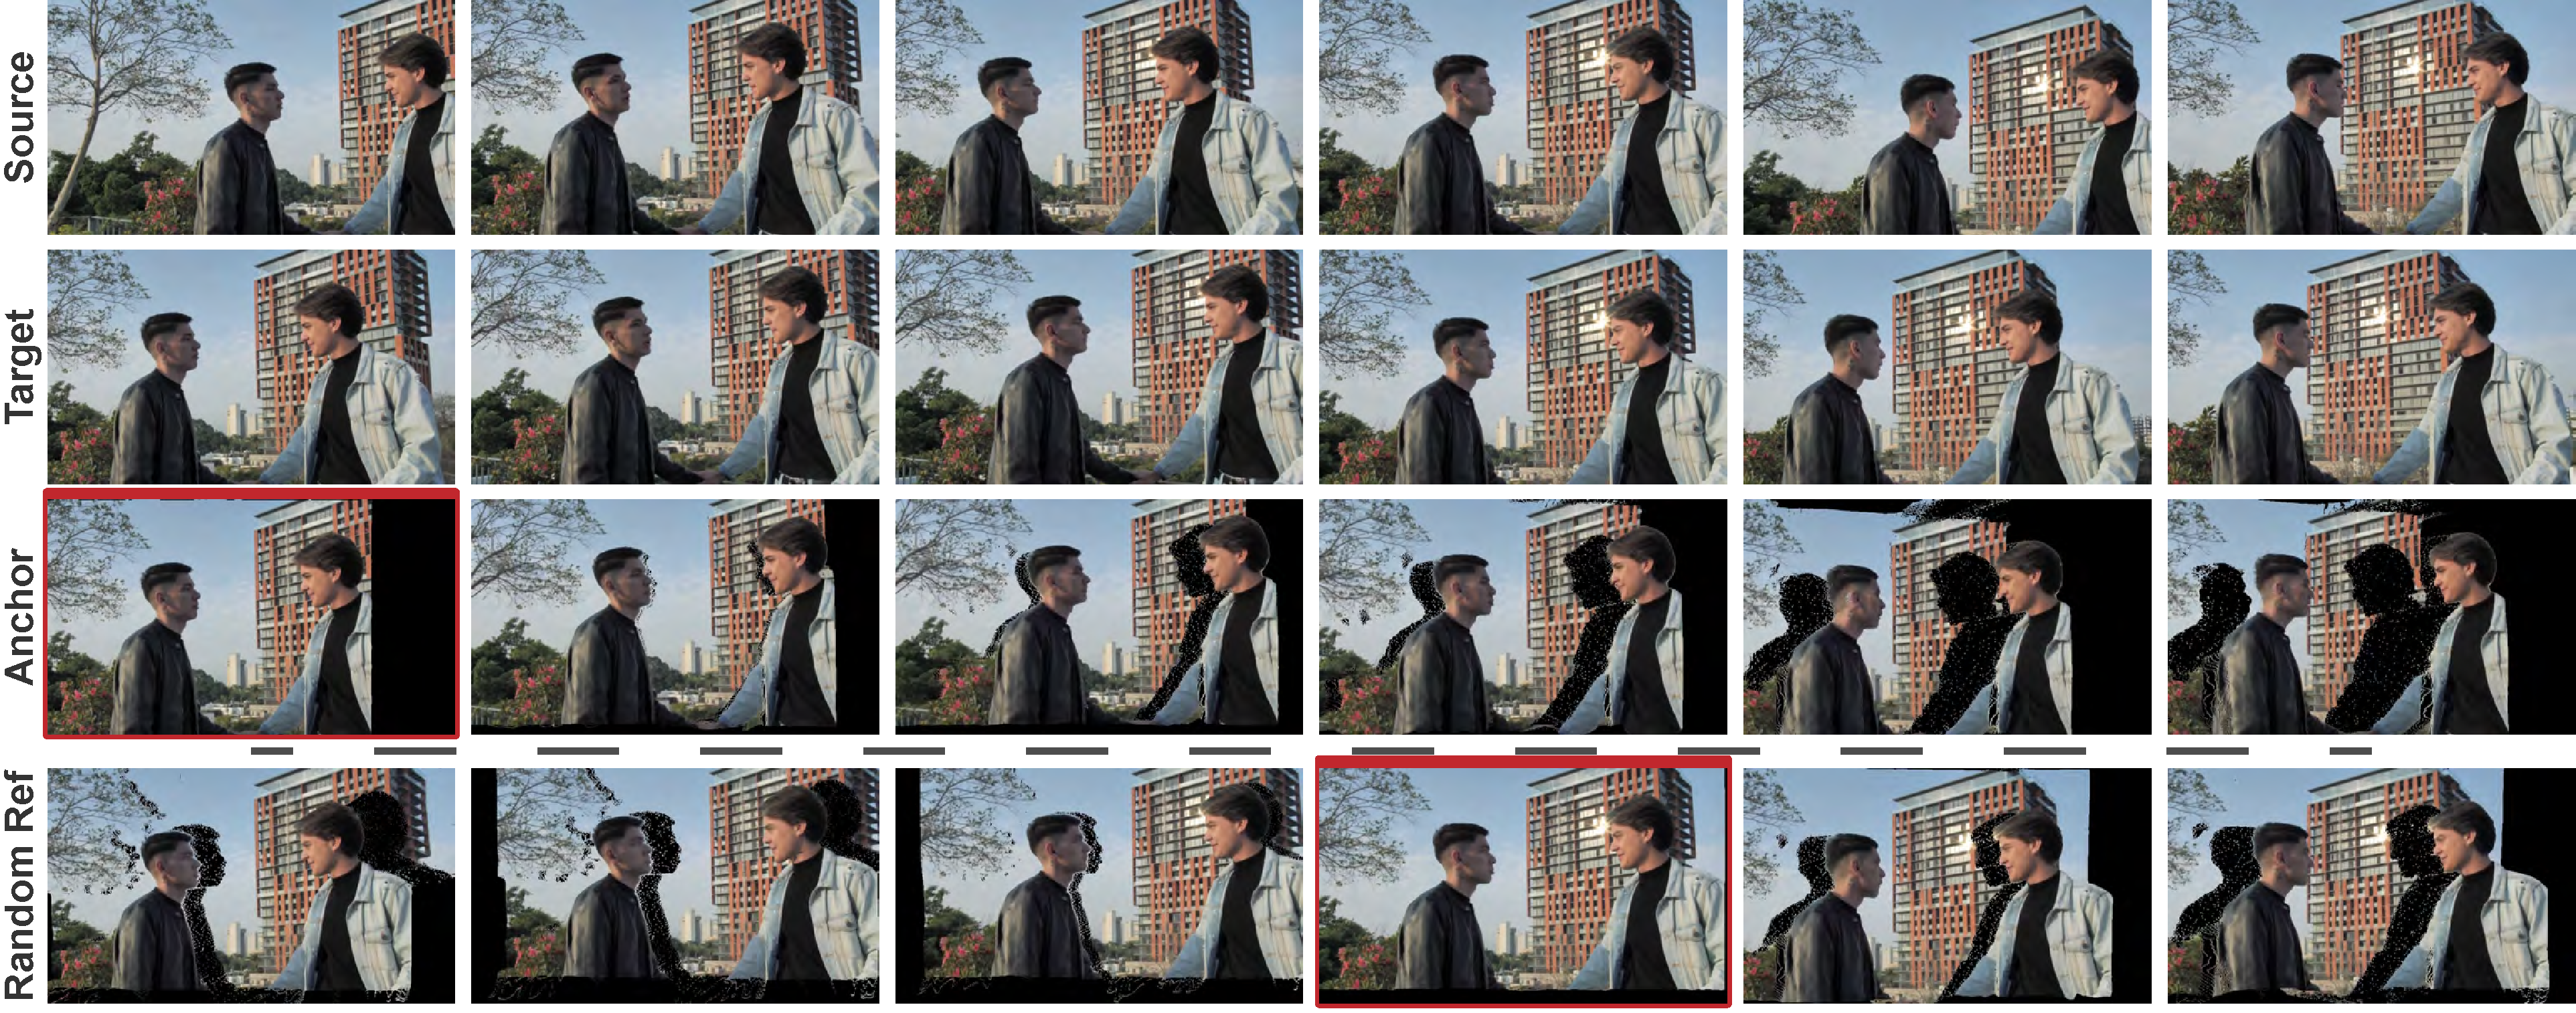
\includegraphics[width=\linewidth]{figures/video_triplets.pdf}
    \vspace{-0.25in}
    \caption{
        \textbf{Our Pseudo Multi-View Triplet and Training Augmentations.}
        \textbf{Top three rows:} Our core training triplet consists of the \textit{Source Video} ($V_s$), the \textit{Target Video} ($V_t$), and the synthetically generated \textit{Anchor Video} ($V_a$). By default, $V_a$ is created by forward-warping a reference frame from $V_s$ to align with the $V_t$ trajectory (using a dense 2D tracker~\cite{4d_recon_harley2025alltracker}). This process incorporates augmentations like 3D-aware noise injection into the reference frame before warping, simulating inference-time artifacts.
        \textbf{Bottom row:} In practice, we randomly select the reference anchor frame for 2D tracking and warping. This reduces overfitting and improves anchor alignment for long sequences.
    }
    \label{fig:triplets}
    \vspace{-0.2in}
\end{figure*}

\subsection{Video-to-Video Generation and Re-shooting}
Camera-controlled video reshooting has been investigated in several recent works, including \recammaster{}~\cite{bai2025recammaster}, \exfd{}~\cite{ex4d}, and \trajectorycrafter{}~\cite{yu2025trajectorycrafter}. Methods relying purely on synthetic video data~\cite{bai2025recammaster, gcd} suffer from an inherent generalization gap. They typically fail on real-world samples or novel object interactions outside their training distribution. However, as we demonstrate, utilizing synthetic data sparingly alongside real-world data provides critical signals for extreme camera translations.

To address the synthetic-to-real gap, other methods employ 4D point tracking and depth estimation on in-the-wild videos~\cite{ex4d,jeong2025reangle,chen2025reconstruct}. Crucially, methods like EPiC~\cite{wang2025epic} rely solely on the projected anchor without querying the full source video. As the camera moves, the anchor accumulates artifacts, forcing the model to overfit to noisy textures and resulting in severe texture drift. Our method fundamentally differs by using the anchor strictly for geometric guidance while actively retrieving clean textures directly from the source video.

Furthermore, dynamic video reshooting must be clearly distinguished from static Novel View Synthesis (NVS). While concurrent self-supervised methods~\cite{mitchel2026true,jiang2025rayzer} excel at static NVS, they inherently fail to handle the non-rigid motion required for complex dynamic scenes. Additionally, while some approaches leverage 360-degree panoramic videos~\cite{xia2025panowan,luo2025beyond} to achieve angular diversity, high-quality dynamic 360-degree datasets remain relatively scarce. Our method instead unlocks the abundance of internet-scale standard perspective videos.

In contrast to existing constraints, our scalable hybrid methodology generates training pairs directly from monocular videos to teach implicit 4D spatiotemporal routing. By co-training this real-world data with a small fraction of multi-view synthetic data, our architectural adaptations facilitate strong alignment with extreme camera trajectories while maintaining high quality textures from source video.